% Libro online bastante completo para consulta de Latex: http://en.wikibooks.org/wiki/LaTeX/
% Versión en castellano: http://es.wikibooks.org/wiki/Manual_de_LaTeX
\documentclass[12pt, a4paper, titlepage]{article}

\usepackage[spanish]{babel} % Soporte multilenguaje para LaTeX.

\usepackage[a4paper, top=2.5cm, bottom=2.5cm, left=2.5cm, right=2.5cm]{geometry} % Interfaz flexible para definir las dimensiones del documento

\usepackage[utf8]{inputenc} % Aceptar diferentes tipos de codificación de caracteres de entrada (en este caso usamos la codificación Unicode UTF-8)

\usepackage{graphicx} % Soporte aumentado para gráficos 
\usepackage{hyperref}

\begin{document}

%%%%%%%%%%%%%%%%%%%%%%%%%%%%%%%%%%%%%%%%%%%%%%%%%%%%%%%%%%%%%%%%%%%%%%%%%%%%%%%%
% PORTADA
%%%%%%%%%%%%%%%%%%%%%%%%%%%%%%%%%%%%%%%%%%%%%%%%%%%%%%%%%%%%%%%%%%%%%%%%%%%%%%%%


\begin{titlepage}


\includegraphics[width=15cm]{Imagenes/Simbolo_logo_UDC.png}

% Lista de tamaños: \Huge, \huge, \LARGE, \Large, \large, \small, \footnotesize, \tiny
\vspace{3cm}

\begin{center}

\includegraphics[scale=0.3]{Imagenes/1a_Practica_ER_14-15.png}
\end{center}


\begin{flushright}
	
	\LARGE{\textbf{ JoinMe!}}
	
	\LARGE{\textbf{Diagramas de Secuencia del Sistema}}
	
	\large{\textbf{Version 1.0}}
	
\end{flushright}

\vspace{1cm}
\begin{center}
José Antonio López Sebio\\
Pablo Paz Varela\\
Grupo ER-12-03\\
\end{center}

\vspace{2cm}

\begin{center}
	\large{\textbf{Histórico}}
	
    \begin{tabular}{ | p{4cm} | p{2cm} | p{6cm} | p{3cm} |}
    \hline
    \textbf{Fecha} & \textbf{Version} & \textbf{Descripción} & \textbf{Autor} \\ \hline
      17/03/2014 & 1.0 & Primera Revisión & ER-12-03\\ \hline
      & 1.1 &  & ER-12-03\\ \hline
     &  & &\\ \hline
    \end{tabular}
\end{center}

\end{titlepage}
\clearpage

%%%%%%%%%%%%%%%%%%%%%%%%%%%%%%%%%%%%%%%%%%%%%%%%%%%%%%%%%%%%%%%%%%%%%%%%%%%%%%%%
% INDICE
%%%%%%%%%%%%%%%%%%%%%%%%%%%%%%%%%%%%%%%%%%%%%%%%%%%%%%%%%%%%%%%%%%%%%%%%%%%%%%%%

\tableofcontents
\clearpage

%%%%%%%%%%%%%%%%%%%%%%%%%%%%%%%%%%%%%%%%%%%%%%%%%%%%%%%%%%%%%%%%%%%%%%%%%%%%%%%%

%%%%%%%%%%%%%%%%%%%%%%%%%%%%%%%%%%%%%%%%%%%%%%%%%%%%%%%%%%%%%%%%%%%%%%%%%%%%%%%%
\section{Introducción}
%%%%%%%%%%%%%%%%%%%%%%%%%%%%%%%%%%%%%%%%%%%%%%%%%%%%%%%%%%%%%%%%%%%%%%%%%%%%%%%%

Este documento proporciona el modelado dinámico de la red social \textbf{JoinMe!} .


%%%%%%%%%%%%%%%%%%%%%%%%%%%%%%%%%%%%%%%%%%%%%%%%%%%%%%%%%%%%%%%%%%%%%%%%%%%%%%%%
\section{Diagramas de secuencia del sistema DSS }
%%%%%%%%%%%%%%%%%%%%%%%%%%%%%%%%%%%%%%%%%%%%%%%%%%%%%%%%%%%%%%%%%%%%%%%%%%%%%%%%

\subsection{CU01 - Registrar usuario}

\subsubsection{Precondiciones}
\begin{enumerate}
	\item El usuario no debe estar registrado en el sistema.
\end{enumerate}

\subsubsection{Diagrama de Secuencia}
\begin{center}
	\includegraphics[width=\textwidth]{Imagenes/registrarUsuario}
\end{center}

\subsubsection{Postcondiciones}
\begin{enumerate}
	\item Los datos del usuario deben quedar registrados en el sistema.
	\item El usuario tiene que poder acceder al sistema.
\end{enumerate}

%%%%%%%%%%%%%%%%%%%%%%%%%%%%%%%%%%%%%%%%%%%%%%%%%%%%%%%%%%%%%%%%%%%%%%%%%%%%%%%%

\subsection{CU03 - Aceptar solicitud de amistad}

\subsubsection{Precondiciones}
\begin{enumerate}
	\item El usuario tiene la sesión iniciada en la red social.
	\item El usuario tiene una solicitud de amistad en su bandeja de notificaciones.
\end{enumerate}

\subsubsection{Diagrama de Secuencia}
\begin{center}
	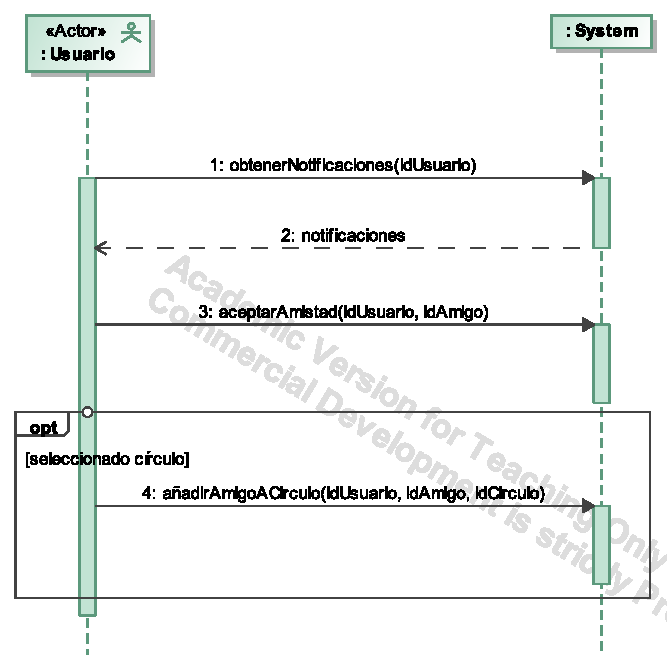
\includegraphics[width=\textwidth]{Imagenes/Aceptar_solicitud_de_amistad}
\end{center}

\subsubsection{Postcondiciones}
\begin{enumerate}
	\item El usuario receptor de la solicitud de amistad y el emisor se hacen amigos en la red social y pueden visitar sus perfiles sin limitaciones.
\end{enumerate}

%%%%%%%%%%%%%%%%%%%%%%%%%%%%%%%%%%%%%%%%%%%%%%%%%%%%%%%%%%%%%%%%%%%%%%%%%%%%%%%%

\subsection{CU04 - Rechazar solicitud de amistad}

\subsubsection{Precondiciones}
\begin{enumerate}
	\item El usuario tiene la sesión iniciada en la red social.
	\item El usuario tiene una solicitud de amistad en su bandeja de notificaciones.
\end{enumerate}

\subsubsection{Diagrama de Secuencia}
\begin{center}
	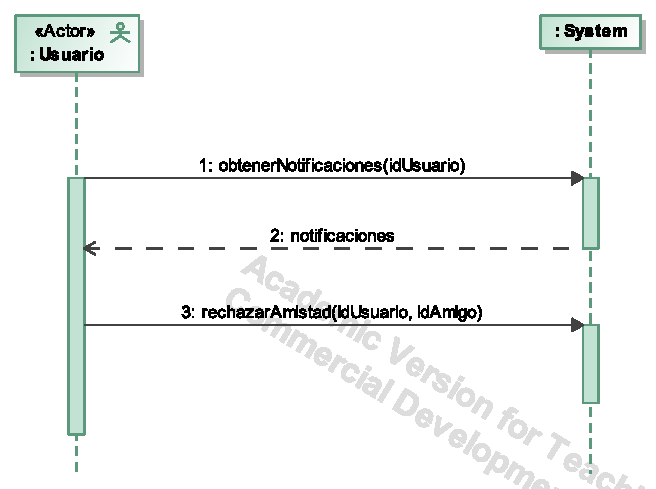
\includegraphics[width=\textwidth]{Imagenes/Rechazar_solicitud_de_amistad}
\end{center}

\subsubsection{Postcondiciones}
\begin{enumerate}
	\item El usuario receptor de la solicitud de amistad y el emisor no se hacen amigos en la red social.
\end{enumerate}

%%%%%%%%%%%%%%%%%%%%%%%%%%%%%%%%%%%%%%%%%%%%%%%%%%%%%%%%%%%%%%%%%%%%%%%%%%%%%%%%

\subsection{CU05 - Ver amigos}

\subsubsection{Precondiciones}
\begin{enumerate}
	\item El usuario tiene la sesión iniciada en la red social.
\end{enumerate}

\subsubsection{Diagrama de Secuencia}
\begin{center}
	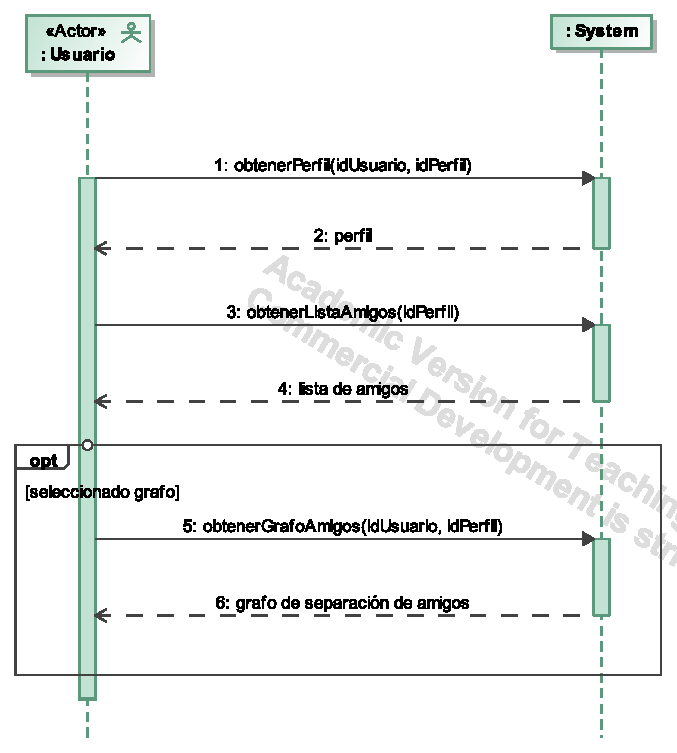
\includegraphics[width=\textwidth]{Imagenes/Ver_amigos}
\end{center}

\subsubsection{Postcondiciones}
\begin{enumerate}
	\item El sistema muestra la lista de amigos.
\end{enumerate}

%%%%%%%%%%%%%%%%%%%%%%%%%%%%%%%%%%%%%%%%%%%%%%%%%%%%%%%%%%%%%%%%%%%%%%%%%%%%%%%%


\subsection{CU06 - Enviar solicitud de amistad}

\subsubsection{Precondiciones}
\begin{enumerate}
	\item El usuario tiene la sesión iniciada en la red social.
	\item El usuario no es amigo del destinatario de la solicitud.
\end{enumerate}

\subsubsection{Diagrama de Secuencia}
\begin{center}
	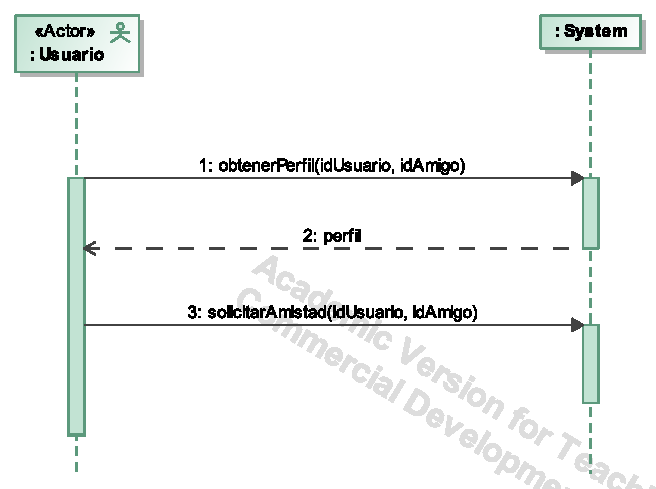
\includegraphics[width=\textwidth]{Imagenes/Enviar_solicitud_amistad}
\end{center}

\subsubsection{Postcondiciones}
\begin{enumerate}
	\item Se le notifica la solicitud al destinatario.
	\item Se agrega a las peticiones de amistad del destinatario.
\end{enumerate}
%%%%%%%%%%%%%%%%%%%%%%%%%%%%%%%%%%%%%%%%%%%%%%%%%%%%%%%%%%%%%%%%%%%%%%%%%%%%%%%%

\subsection{CU11 - Crear entrada}

\subsubsection{Precondiciones}
\begin{enumerate}
	\item El usuario tiene la sesión iniciada en la red social.
\end{enumerate}


\subsubsection{Diagrama de Secuencia}
\begin{center}
	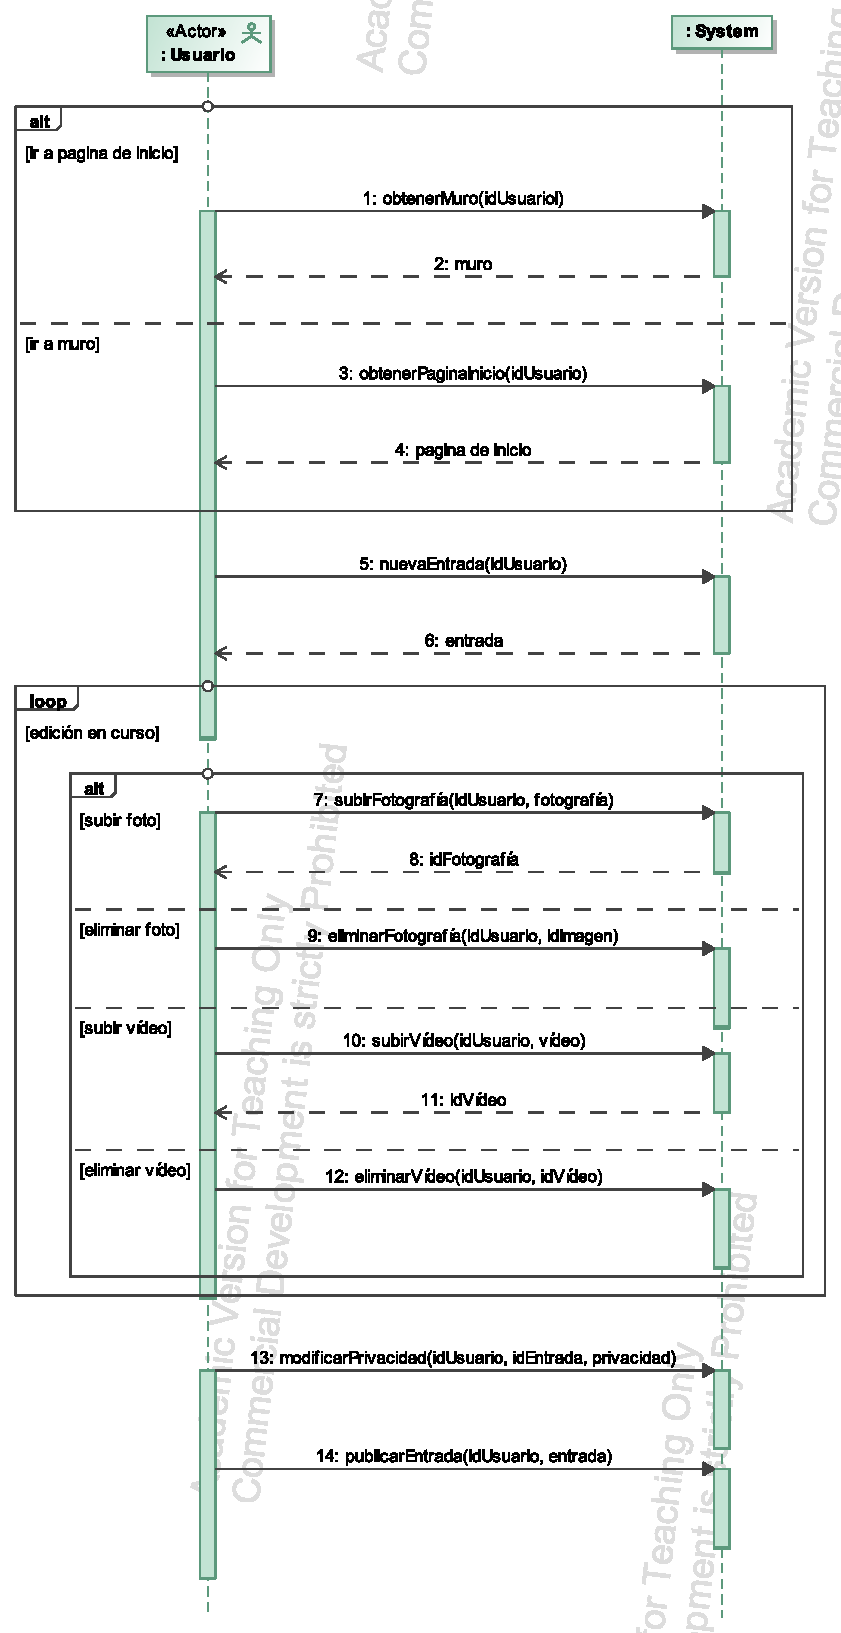
\includegraphics[scale=0.85]{Imagenes/Crear_entrada}
\end{center}	


\subsubsection{Postcondiciones}
\begin{enumerate}
	\item La entrada queda almacenada y agregada al muro del usuario.
\end{enumerate}



\end{document}